\noindent{\normalsize \textbf{IntelliJ IDEA:}}
\begin{itemize}
\item IntelliJ IDEA là môi trường phát triển tích hợp (IDE) đầu tiên do JetBrains phát triển, được thiết kế chủ yếu cho các công nghệ dựa trên JVM như Java, Groovy, Kotlin và Scala, đồng thời hỗ trợ Java EE và phát triển web. Phiên bản đầu tiên của IntelliJ IDEA được phát hành vào tháng 1 năm 2001. Trong dự án Instagram clone, công cụ này được sử dụng để viết mã và phát triển API backend bằng Spring Boot, giúp tăng hiệu suất lập trình với các tính năng như gợi ý mã thông minh, kiểm tra lỗi, và tích hợp công cụ quản lý dự án.

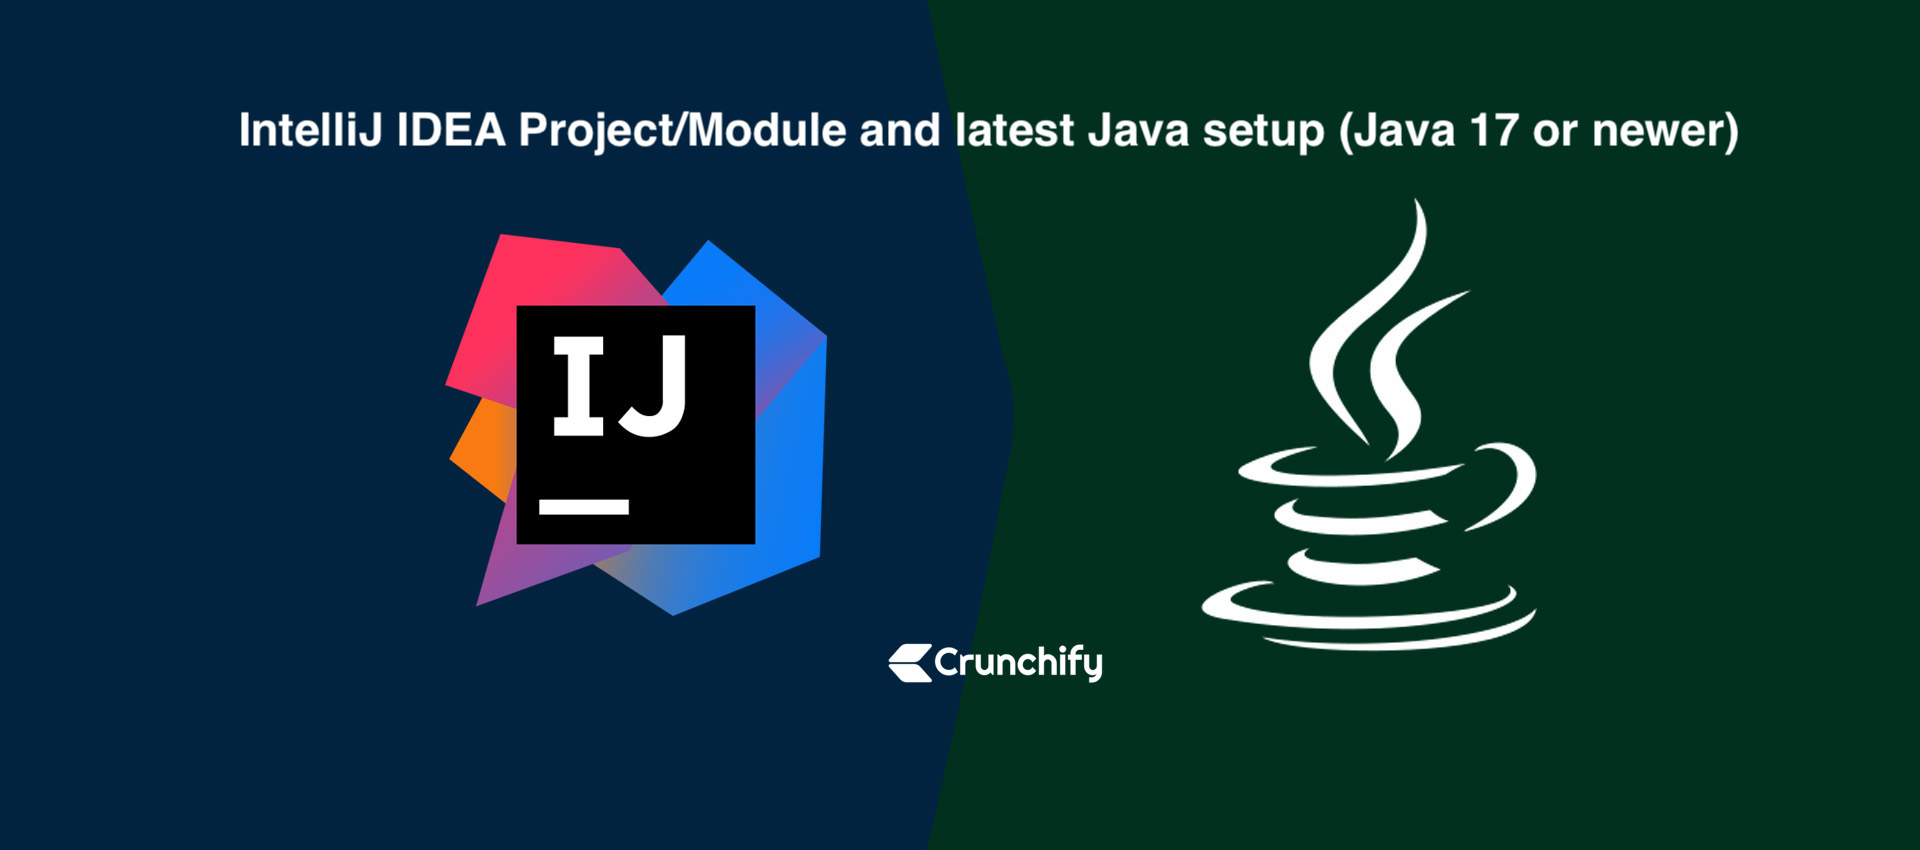
\includegraphics[width=\textwidth]{img/intelij.png}
\end{itemize}


\noindent{\normalsize \textbf{Visual Studio Code (VS Code):}}
\begin{itemize}
\item Visual Studio Code là một trình soạn thảo mã nguồn nhẹ nhưng mạnh mẽ, hỗ trợ đa nền tảng như Windows, macOS và Linux. Với các tính năng như hoàn thành mã thông minh, tích hợp Git, và hỗ trợ nhiều tiện ích mở rộng, VS Code được sử dụng để phát triển frontend của dự án Instagram clone với ReactJS. Công cụ này giúp lập trình viên dễ dàng viết mã, gỡ lỗi, và quản lý các thư viện như Ant Design, Redux, và TailwindCSS một cách hiệu quả.
\end{itemize}

\noindent{\normalsize \textbf{Postman:}}
\begin{itemize}
\item Postman là một công cụ phổ biến được sử dụng để kiểm thử và làm việc với các API, đặc biệt là API kiểu REST. API đóng vai trò quan trọng trong việc kết nối các thành phần của ứng dụng, và Postman giúp đơn giản hóa quá trình gọi và kiểm tra API mà không cần viết mã. Công cụ này hỗ trợ tất cả các phương thức HTTP như GET, POST, PUT, PATCH, DELETE, và cho phép lưu lại lịch sử các yêu cầu (request) để sử dụng lại khi cần. Trong dự án Instagram clone, Postman được sử dụng để kiểm tra các API như đăng bài post (POST /api/post), lấy danh sách bài post (GET /api/post), và gửi tin nhắn.
\end{itemize}

\noindent{\normalsize \textbf{MySQL Workbench:}}
\begin{itemize}
\item MySQL Workbench là một công cụ quản lý cơ sở dữ liệu MySQL, cung cấp giao diện đồ họa để phát triển, thiết kế và quản lý cơ sở dữ liệu một cách trực quan. Công cụ này cho phép dễ dàng tạo, chỉnh sửa cơ sở dữ liệu, thực hiện các thao tác như đảo ngược (reverse engineering) để tạo mô hình từ cơ sở dữ liệu hiện có, và chuyển tiếp (forward engineering) để triển khai mô hình thành cơ sở dữ liệu. Trong dự án Instagram clone, MySQL Workbench được sử dụng để thiết kế và quản lý cơ sở dữ liệu MySQL, bao gồm các bảng như users, posts, comments, và messages.

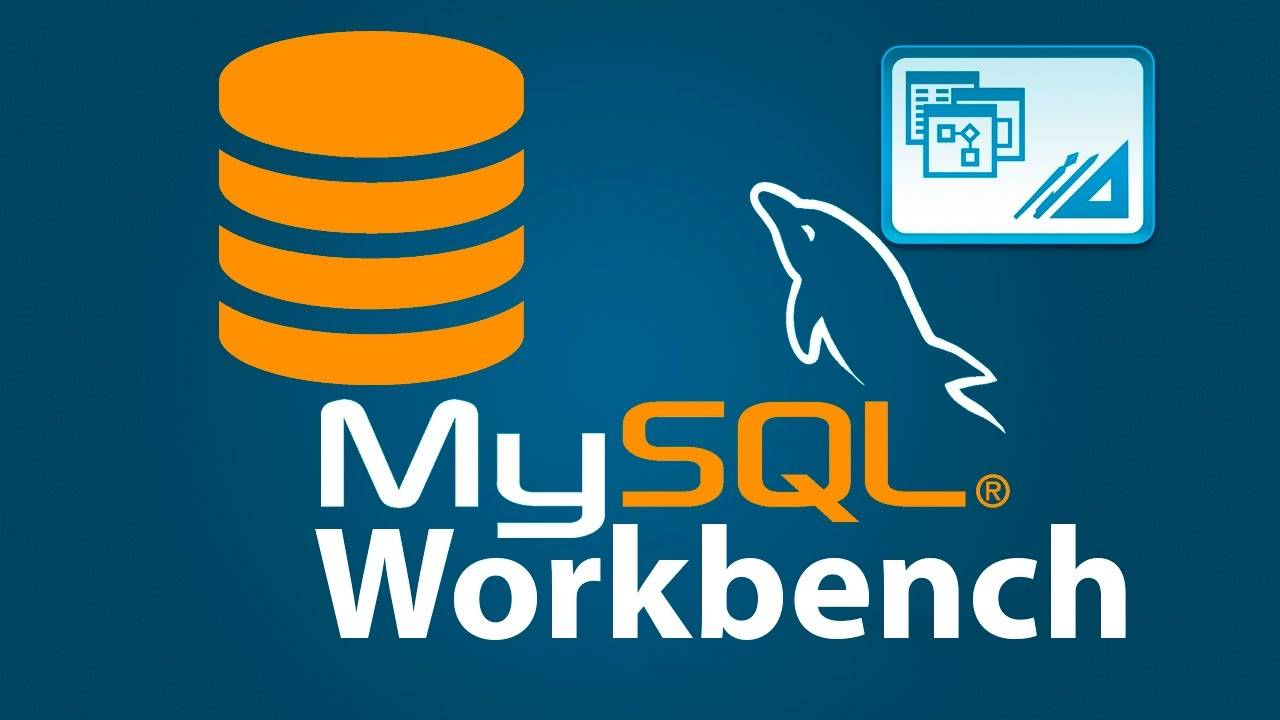
\includegraphics[width=\textwidth]{img/mysql_workbench.png}
\end{itemize}

\noindent{\normalsize \textbf{GitHub:}}
\begin{itemize}
\item GitHub là một nền tảng quản lý mã nguồn phổ biến, cho phép các lập trình viên chia sẻ, cộng tác và quản lý phiên bản mã nguồn một cách hiệu quả. Sự phát triển của GitHub bắt đầu vào ngày 19 tháng 10 năm 2007, và trang web chính thức được ra mắt vào tháng 4 năm 2008 bởi Tom Preston-Werner, Chris Wanstrath, và PJ Hyett. Microsoft đã mua lại GitHub vào tháng 6 năm 2018. Trong dự án Instagram clone, GitHub được sử dụng để lưu trữ mã nguồn, quản lý phiên bản, và hỗ trợ làm việc nhóm giữa các thành viên phát triển frontend và backend.
\end{itemize}